% !TEX root = ../main.tex

\section{Results}
\label{sec:results}

Figure~\ref{fig:example} shows the measured signal together with the model of Equation~\ref{eq:model}.

% A figure "floats": LaTeX places it where it fits best, near here.
% [tb] means "top or bottom of a page". The picture file lives in the
% figures/ folder; drag your own images into the project and change
% the file name to use them.
\begin{figure}[tb]
  \centering
  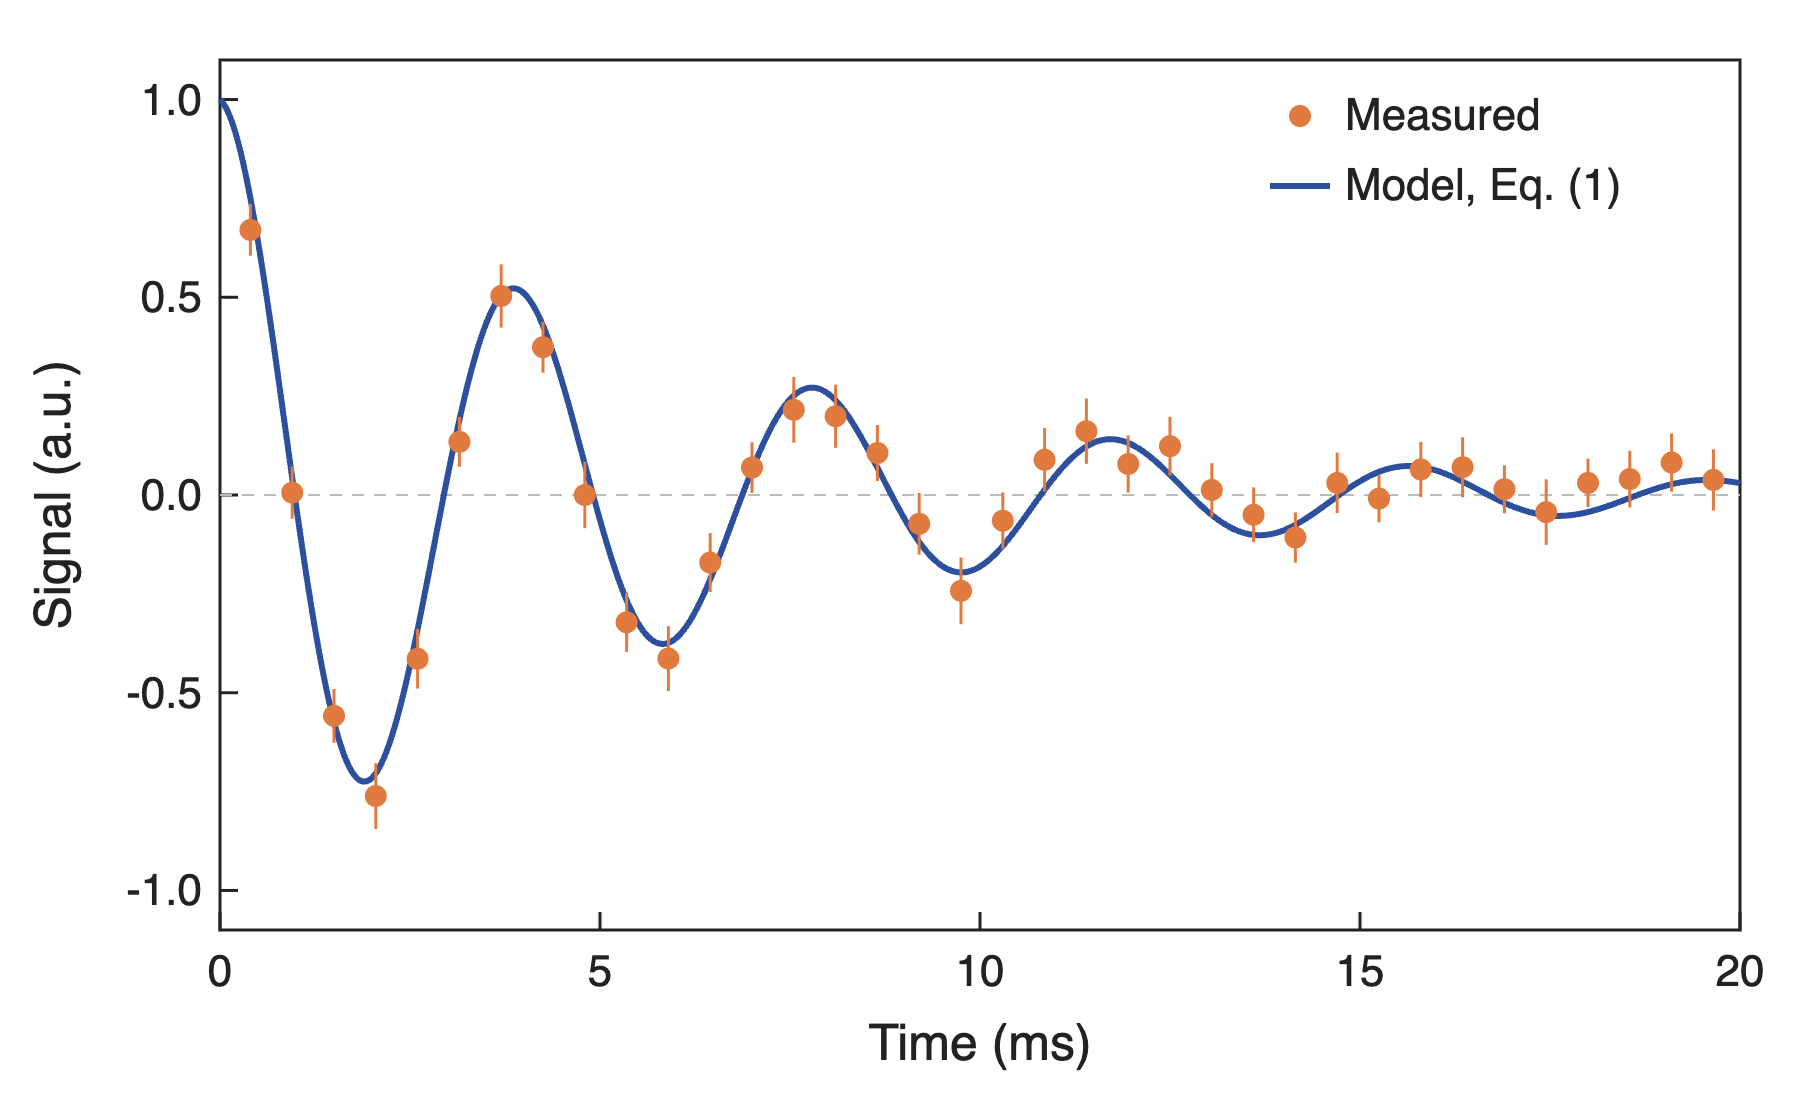
\includegraphics[width=0.75\linewidth]{figures/example-plot.png}
  \caption{Measured signal (points) and the damped-oscillation model of Equation~\ref{eq:model} (line). The caption goes under the picture.}
  \label{fig:example}
\end{figure}

Tables are built from rows: \verb|&| separates columns and \verb|\\| ends a row.
Table~\ref{tab:samples} lists the samples.

\begin{table}[tb]
  \centering
  \caption{Samples used in this study. Table captions usually go above the table.}
  \label{tab:samples}
  \begin{tabular}{lcc}
    \toprule
    Sample & Thickness (nm) & Decay time $\tau$ (ms) \\
    \midrule
    A & 12 & 3.1 \\
    B & 25 & 4.7 \\
    C & 40 & 6.2 \\
    \bottomrule
  \end{tabular}
\end{table}

Double-click anywhere in the PDF and OpenTex jumps to the matching line here.
Press Ctrl/Cmd+J in the source to jump the other way.
